\section{Google Classroom (https://classroom.google.com/)}
Google Classroom is an online learning management tool provided by Google which offers a free and easy tool for helping educators manage and assess progress of students. It has become one of the most popular learning management platforms adopted in schools across Australia. 
The main selling points of this platform are:
\begin{itemize}
    \item The ability to easily manage students learning:
    \begin{itemize}
        \item Allowing students to join classes directly or by sharing a code or link;
        \item Setup a class quickly and create class work that is displayed on students’ calendars; and, 
        \item Providing communication with students’ guardians and automatically sending them updates.
    \end{itemize}
    \item The ability to easily measure student progress:
    \begin{itemize}
        \item Storing frequently used feedback to be used for fast and personalised responses;
        \item Allowing teachers to grade consistently and transparently with rubric integrated student work; and,
        \item Providing students with a plagiarism checker to help them produce their own original work.
    \end{itemize}
    \item The ability to provide collaboration between students and teachers:
    \begin{itemize}
        \item Connecting students and teachers online in virtual classes;
        \item Allowing communication of announcements on the Stream page; and,
        \item Enabling face to face connections with students using Google Meet.
    \end{itemize}
    \item Keeping data secure: 
    \begin{itemize}
        \item Authenticating users through a login feature;
        \item Restricting classroom activities to members; and,
        \item Assuring data is never used for advertising purposes.
    \end{itemize}
    \item Allowing for third party apps to be integrated in learning for example:
    \begin{itemize}
        \item Schoolytics (https://www.schoolytics.io/): Allows educators and teachers to generate insights on student learning; and,
        \item Studyo (https://studyo.co/): Provides educators and students with more comprehensive planning tools.
    \end{itemize}
\end{itemize}

\subsection{Features}
Google classroom provides all of the basic functionalities and some unique features of a learning management system.
\begin{itemize}
    \item Allows teachers to create classes/groups which students can join through a link or code;
    \item Allows users to create announcements in which others can comment within the class;
    \item Allows teachers to create classwork by creating questions, assignments, quizzes or class material;
    \item Classwork can be scheduled and the due dates of the classwork will show up on students’ calendars;
    \item Classwork, posts and announcements can be reused;
    \item Other Google applications (e.g. Google Drive, Google Docs, Google Sheets, Google Presentations and Google Meet) are integrated within Google Classroom, offering more utility for all users; and,
    \item Allows teachers to input grades which are viewable by students
\end{itemize}

\newpage

\subsection{Review}

In terms of the aspect of ease of use, flexibility and usability, Google Classroom offers teachers to reuse questions or sets of questions for classwork.
Figure 2.1 highlights the functionality that allows teachers to reuse classwork. 
While reusing classwork, teachers are able to then set separate parameters such as the due date, add more questions, change the topic and change mark allocation.

\begin{figure}[h]
    \centering
    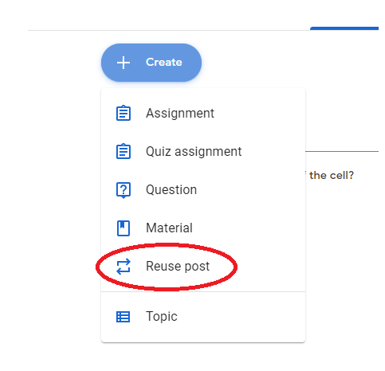
\includegraphics[scale=0.5]{reuse_post}
    \caption{Teachers can reuse posts.}
\end{figure}

Topics can also be created in Google Classroom.
Topics allow for categorisation of class work. 
An example of the topics is shown in Figure 2.2. 
The example displays 2 topics, each with 1 question. 
One functionality that is not implemented is the use of prerequisites for topics. 
For example, if topic1 was a prerequisite for topic2, then students who have not completed topic1 cannot access topic2. 
This design does not show how each topic is linked with each other which could be improved on.

\begin{figure}[h]
    \centering
    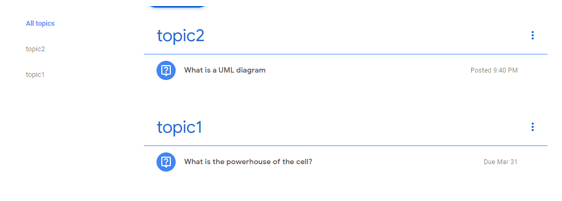
\includegraphics[scale=0.5]{topics}
    \caption{List of topics.}
\end{figure}

One interesting feature within Google Classroom is the integration of other first party applications such as Google Calendar and Google Drive. 
Google Calendar is a very popular task reminder and calendar application and would benefit greatly with the incorporation of displaying due dates for classwork from Google Classroom. 
Google Calendar allows for the easy visualisation of important dates and thus is suitable for Google classroom. 
Google Drive is also a very popular file hosting server where files can be easily shared with other people. 
For the case of Google Classroom, it can be utilised to share classwork with students.

\begin{figure}[h]
    \centering
    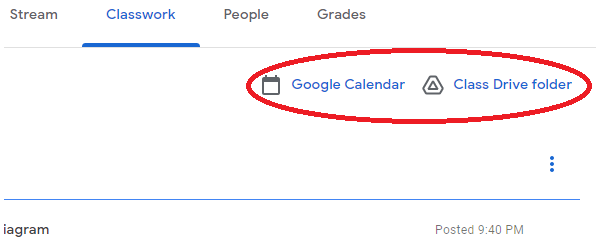
\includegraphics[scale=0.5]{google-apps}
    \caption{Google Drive and Google Calendars are integrated.}
\end{figure}

Due to Google Classroom being affiliated with Google many of the other platforms related to Google are integrated very well. 
Announcements can be created which have Google Drives and YouTube videos attached which further improve the usability of Google Classroom.

\begin{figure}[h]
    \centering
    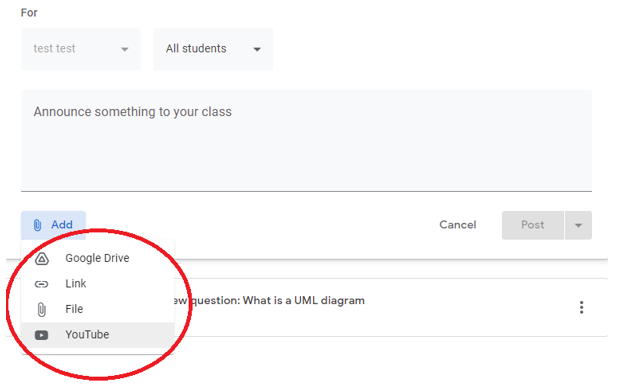
\includegraphics[scale=0.5]{youtube}
    \caption{Google Drive and YouTube are integrated}
\end{figure}

Overall Google Classroom does not have many unique features that make it an outstanding learning management platform; however, it does provide the integration of other Google platforms such as Google Drive, Google Calendars, Google Docs, Google Sheets, Google Presentations and YouTube.
